\documentclass[onecolumn, draftclsnofoot,10pt, compsoc]{IEEEtran}
\usepackage{graphicx}
\usepackage{url}
\usepackage{float}
\usepackage{setspace}

\usepackage[colorinlistoftodos]{todonotes}%Take out when complete, allows intext comments during work

\usepackage{geometry}
\geometry{textheight=9.5in, textwidth=7in}

% Used for code listings
\usepackage{listings}
\usepackage{color}

\definecolor{dkgreen}{rgb}{0,0.6,0}
\definecolor{gray}{rgb}{0.5,0.5,0.5}
\definecolor{mauve}{rgb}{0.58,0,0.82}

\lstset{frame=tb,
  language=[Sharp]C,
  aboveskip=3mm,
  belowskip=3mm,
  showstringspaces=false,
  columns=flexible,
  basicstyle={\small\ttfamily},
  numbers=none,
  numberstyle=\tiny\color{gray},
  keywordstyle=\color{blue},
  commentstyle=\color{dkgreen},
  stringstyle=\color{mauve},
  breaklines=true,
  breakatwhitespace=true,
  tabsize=3
}

% 1. Fill in these details
\def \CapstoneTeamName{		Team Sandy}
\def \CapstoneTeamNumber{		44}
\def \GroupMemberOne{			Raja Petroff			}
\def \GroupMemberTwo{			Andrew Soltesz			}
\def \GroupMemberThree{			Mark Sprouse}
\def \CapstoneProjectName{		AR Sandbox for Construction Planning}
\def \CapstoneSponsorCompany{	Oregon State University}
\def \CapstoneSponsorPerson{		Dr. Joseph Louis}
\title{Progress Report}

% 2. Uncomment the appropriate line below so that the document type works
\def \DocType{		%Problem Statement
				%Requirements Document
				%Technology Review
				%Design Document
				Progress Report
				}
			
\newcommand{\NameSigPair}[1]{\par
\makebox[2.75in][r]{#1} \hfil 	\makebox[3.25in]{\makebox[2.25in]{\hrulefill} \hfill		\makebox[.75in]{\hrulefill}}
\par\vspace{-12pt} \textit{\tiny\noindent
\makebox[2.75in]{} \hfil		\makebox[3.25in]{\makebox[2.25in][r]{Signature} \hfill	\makebox[.75in][r]{Date}}}}
% 3. If the document is not to be signed, uncomment the RENEWcommand below
\renewcommand{\NameSigPair}[1]{#1}

%%%%%%%%%%%%%%%%%%%%%%%%%%%%%%%%%%%%%%%
\begin{document}
\begin{titlepage}
    \pagenumbering{gobble}
    \begin{singlespace}
    	
\includegraphics[height=4cm]{coe_v_spot1}
        \hfill 
        % 4. If you have a logo, use this includegraphics command to put it on the coversheet.
        %\includegraphics[height=4cm]{CompanyLogo}   
        \par\vspace{.2in}
        \centering
        \scshape{
            \huge CS Capstone \DocType \par
            {\large\today}\par
            \vspace{.5in}
            \textbf{\Huge\CapstoneProjectName}\par
            \vfill
            {\large Prepared for}\par
            \Huge \CapstoneSponsorCompany\par
            \vspace{5pt}
            {\Large\NameSigPair{\CapstoneSponsorPerson}\par}
            {\large Prepared by }\par
            Group\CapstoneTeamNumber\par
            % 5. comment out the line below this one if you do not wish to name your team
            %\CapstoneTeamName\par 
            \vspace{5pt}
            {\Large
                \NameSigPair{\GroupMemberOne}\par
                \NameSigPair{\GroupMemberTwo}\par
                \NameSigPair{\GroupMemberThree}\par
            }
            \vspace{20pt}
        }
        \begin{abstract}
        % 6. Fill in your abstract
        This document covers the progress made on the Augmented Reality Sandbox capstone project up to the first half of spring term of the 2017-2018 school year. Specifically, this document recaps the scope of the project, discusses the current state of the project, discusses problems encountered thus far, and discusses interesting code used in the project.
        \end{abstract}     
    \end{singlespace}
\end{titlepage}
\newpage
\pagenumbering{arabic}
\tableofcontents
% 7. uncomment this (if applicable). Consider adding a page break.
%\listoffigures
%\listoftables
\clearpage

% 8. now you write!
\section{Project Recap} %Raja
The purpose of this project is to create an augmented reality (AR) sandbox for construction planning.
This AR sandbox will greatly enhance the ability of engineers to collaborate, plan, communicate, and learn about these civil concepts in a convenient manner.
It will also give construction engineering students a hands-on approach when learning about important concepts that are involved in construction planning, such as how to calculate the cut and fill of a road.

\par Our goal is to have a working AR sandbox with a road editing feature.
This will allow engineers to manipulate both the terrain, represented by the sand, and the layout of a highway or roadway, represented by a graphic projected onto the sand.
The AR sandbox will also calculate the cut and fill of the road automatically, giving engineers a rough estimate of the amount of material that will need to be moved to build a road.

\begin{figure}[H]
	\centering
	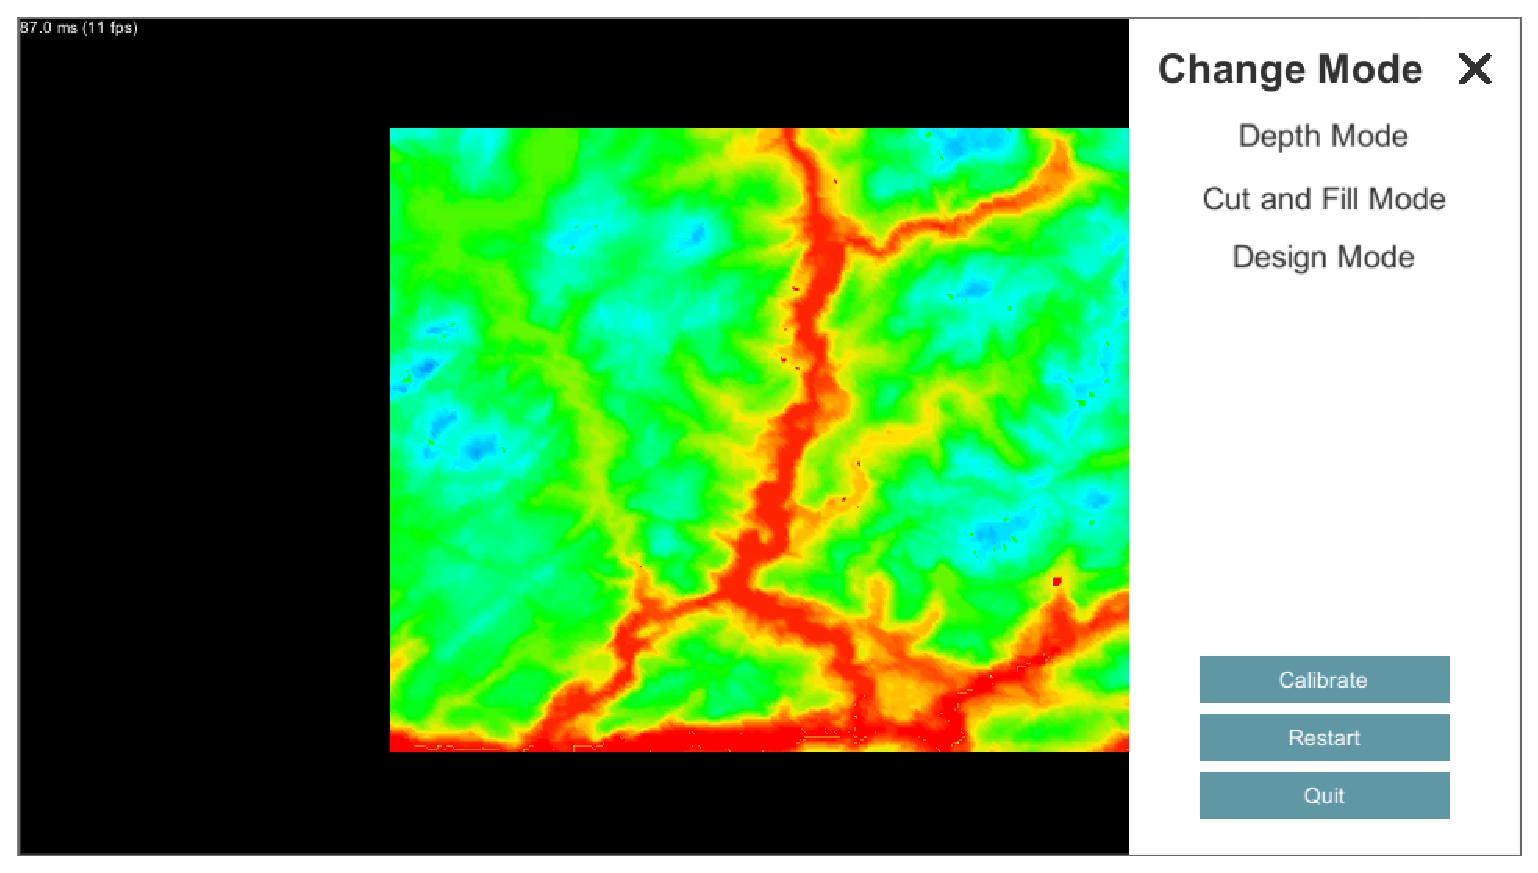
\includegraphics[width=1.\textwidth]{UI}
	\caption{A screenshot of the UI of our software with each of the buttons that correspond to a given mode.}
	\label{fig:UI}
\end{figure}

\section{Project Position} 

Currently, the AR sandbox is feature complete and completely usable. At this point in time, the Kinect is able to capture height data, which is displayed by the system in near real time. Latency is slightly noticeable, but is not a hindrance to usability. 

Depth mode simply colors the terrain and projects this colored map back onto the sand. This mode is complete and will not see any further revisions.

Cut and fill mode is far more efficient and now updates at the same rate as the rest of the system (an improvement over the prior 5 second latency.) The cut and fill table currently only displays the amount of earth that needs to be moved at each station along the road segment, however will display additional information before the full release.

Design mode allows the user to specify a road segment by dragging control points around the sand box area. Control points are now bounded to the edges of the sandbox, and can be transformed in all three dimensions. In order to aid in visualizing the height of the road in relation to the terrain, a cross sectional view has been created, showing the height of the terrain below a given point along the road. An undo system will need to be implemented before the full release, however given the current architecture of the system, this will be relatively trivial.

\begin{figure}[H]
	\centering
	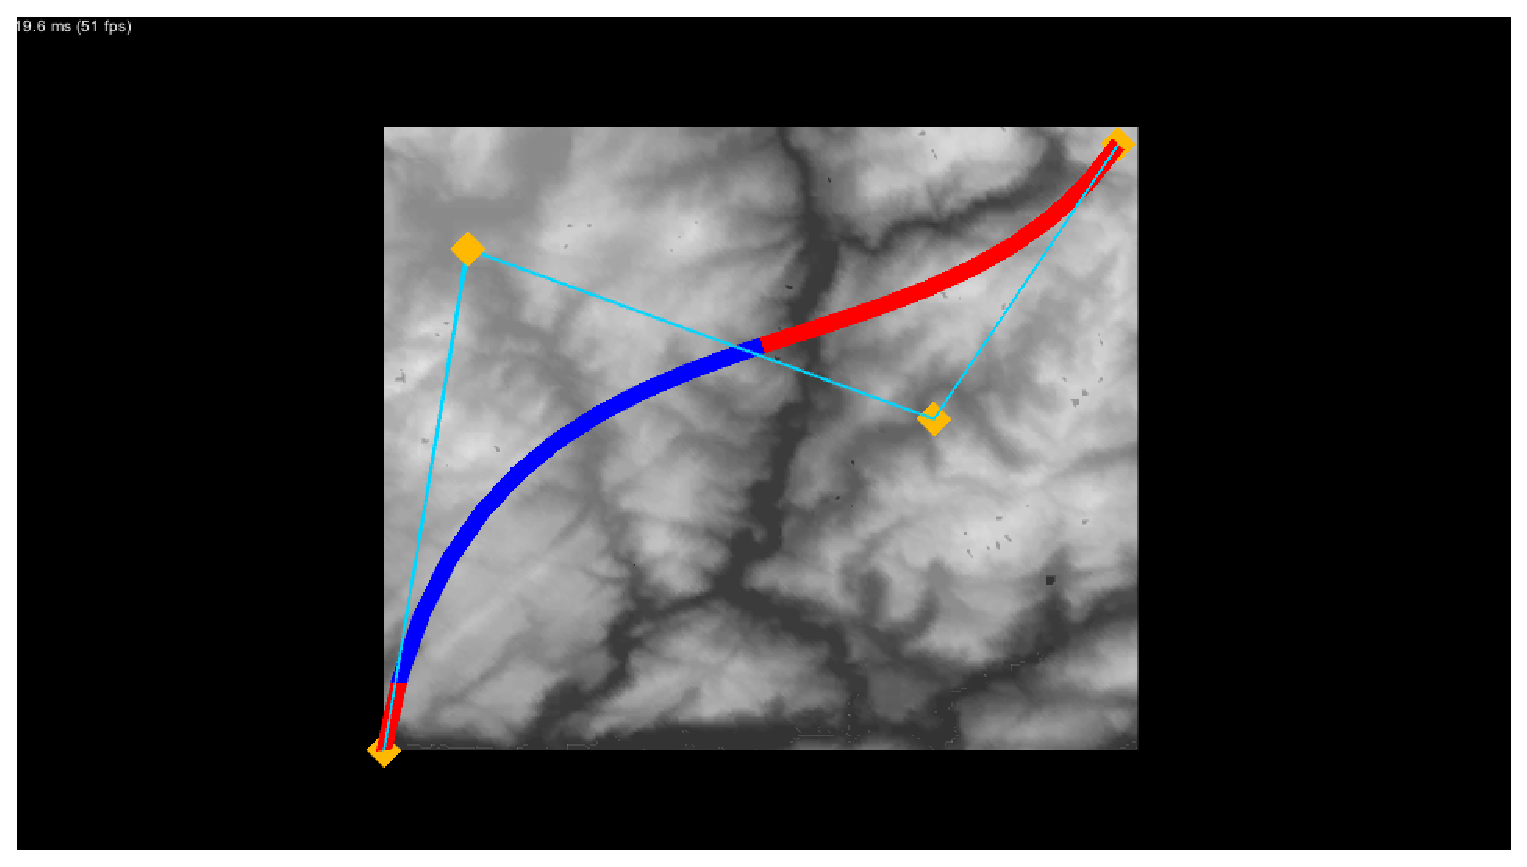
\includegraphics[width=1.\textwidth]{road}
	\caption{An example of what design mode looks like.}
	\label{fig:road}
\end{figure}

Calibration mode allows the bounds of the sandbox to be set using four draggable handles. Additionally, the minimum and maximum depth can be set using a pair of sliders, and the system's units and scale can be set using a dropdown menu. Since the last version, the ability to transform and scale the terrain mesh from within the system has been implemented, giving the user more control over the calibration of the sandbox.

\begin{figure}[H]
	\centering
	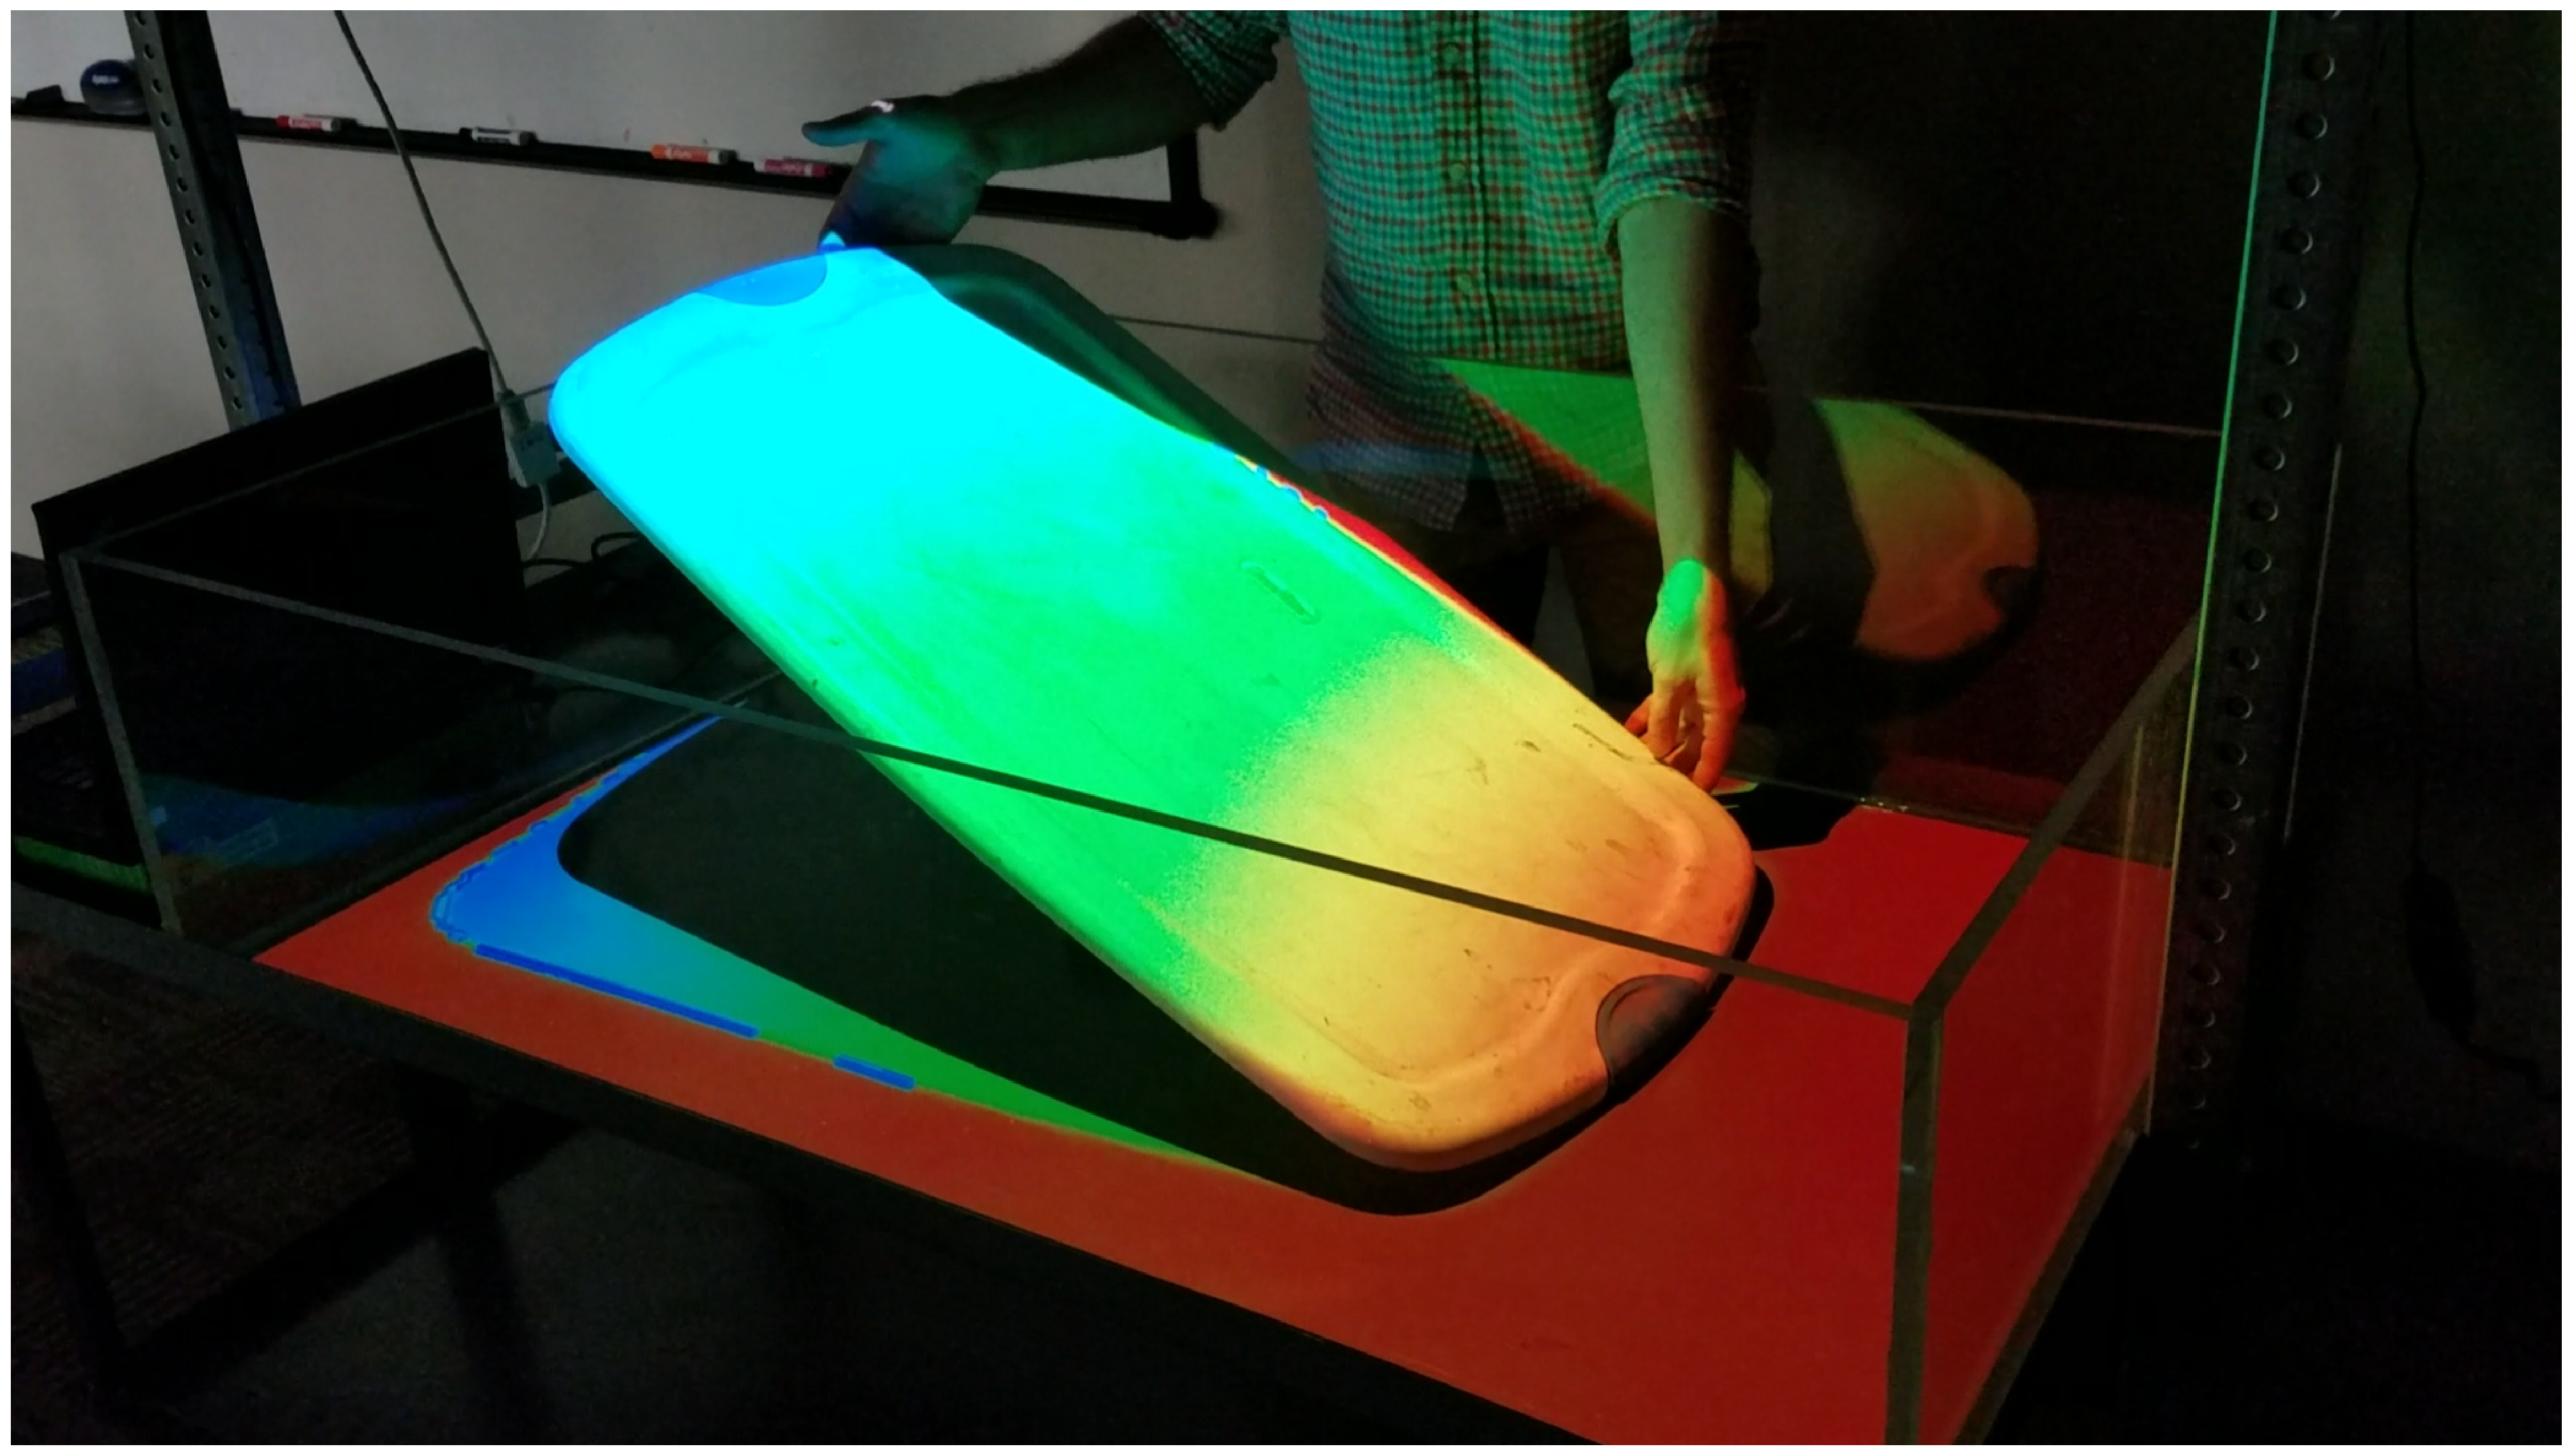
\includegraphics[width=1.\textwidth]{Sandbox_Gradient}
	\caption{A demonstration of the Gradient created with height within the AR Sandbox.}
	\label{fig:Sandbox_Gradient}
\end{figure}

\section{Encountered Problems} %Mark
Similar to previous times, we haven't had a ton of problems.  
With that being said, the few problems we encountered were relatively impactful and/or were unavoidable.  
The first of these noteworthy problems was just illness.  There were several times that a member got sick for a day or two, making them unable to get very much work done on the project.
This is something that is relatively unavoidable (other than just trying to be a healthy person in general).
The only real avoidance is making sure that we have enough time to make up for any time lost do to illness.
For the most part, we did have adequate time to compensate, but sickness did lead to some "crunch-times" that would have been nice to avoid.
\par
The second noteworthy problem that occurred was with the hardware of the sandbox. 
For starters, there was a relatively long time where our team was waiting for the box to be built. 
During this time we were able to keep developing software for the system, but we were unable to truly test things on the system as a whole.
Once the box was actually built, we also encountered a few problems in the mounting system for the projector.
We had failed to realize that the projector projects up at and angle. 
This makes sense when the projector is on a table and needs to project up to a screen, but with it mounted vertically, facing down, its projection was way off center.
Our solution to this was to modify the mounting system such that the projector is displaced from the center of the box by an amount that allows the image to properly align itself.
\par
The last noteworthy issue we had was scheduling meeting times.
At almost all times, at least one person in the group would be unavailable to meet.
In addition, Mark had his bike stolen part into the term which made it that much harder for him to maneuver about and make it to meetings.
To remedy this we had more online meetings and moved any meeting that needed to be in person to less convenient times that we could all make.

\section{Interesting Code}

\begin{lstlisting} [caption=The Bezier curve calculation used for specifying a road path., label=lst:bezier,captionpos=b]
	Vector3 CalculateBezier(float t, List<RoadControlPoint> points) {
		int count = points.Count;
		if (count > 2) {
			return (1 - t) * CalculateBezier(t, points.GetRange(0, count - 1)) + t * CalculateBezier(t, points.GetRange(1, count - 1));
		} else {
			return Vector3.Lerp (points [0].transform.position, points [1].transform.position, t);
		}
	}
\end{lstlisting}

The \texttt{CalculateBezier()} function takes a float \texttt{t} representing the position along the line to sample, and a list of control points that will define the line. The output of this function is a \texttt{Vector3} representing the position in world space at \texttt{t}. The function can support n control points, and works recursively to determine the position.
\\
\begin{lstlisting} [caption=The functionality responsible for translating a Kinect height value to world space., label=lst:getheight,captionpos=b]
	public float GetHeightAtWorldPosition(Vector3 pos) {
		ushort[] heightData;
		heightData = manager.GetData ();

		Vector3 modelPos = pos - transform.position;
		Vector3 texelPos = modelPos / spacing;

		if (texelPos.x >= 0 && texelPos.x < frameWidth && texelPos.z >= 0 && texelPos.z < frameHeight) {
			float y = heightData [((int)texelPos.z) * frameWidth + ((int)texelPos.x)];
			return (((float)y - maxHeight) / (minHeight - maxHeight)) * magnitude;
		} else {
			Debug.LogError ("TerrainGenerator: Request for height data returned 0, world position out of range");
			return 0;
		}
	}
\end{lstlisting}

The \texttt{GetHeightAtWorldPosition()} function takes a world position as a \texttt{Vector3} and returns the height of the terrain at that position. This is accomplished by first converting \texttt{pos} from world coordinates to model coordinates, then determining what texel this position is associated with. Then, since height data comes from the sensor as a 1 dimensional array, the index of the texel must be determined so that its value can be returned.

\newpage

\begin{lstlisting}[caption=A code snippet from the cut and fill manager demonstrating how cut and fill calculations work., label=lst:cutfill,captionpos=b]
public float[] getRoadAreas()
{
    Vector3[] positions = roadPoint.GetRoadPoints();

    float[] roadHeight = new float[roadPoint.GetNumRoadPoints()];
    float[] roadAreas = new float[roadPoint.GetNumRoadPoints()];
    int count = 0;

    foreach (Vector3 p in positions)
    {
        roadHeight[count] = 10f * terrainHeight.GetHeightAtWorldPosition(p);
        roadAreas[count] = (float)(2f * (.5 * roadHeight[count] * roadHeight[count]) + 120f * roadHeight[count]);
        count++;
    }

    return roadAreas;
}
\end{lstlisting}

The \texttt{getRoadAreas()} function returns the cut and fill areas of the road. This is done by first retrieving the points that make up the road, as shown in the \texttt{positions} array. Then, a for-each loop retrieves the height of each road point and then uses it to calculate the area. Once this is finished, the area values are stored in an array called \texttt{roadAreas} and returned to the calling function.

%\appendix

\end{document}